\documentclass[A4,svgnames,9pt,aspectratio=169]{beamer}
%% document options:
%% - aspectratio = { 43, 169, 1610 }
%% - utf8
%%

%%
%% insert list of packages
%%
\usepackage{pgfplots}
\pgfplotsset{compat=1.17}

%% \usepackage[english,french]{babel}

\hypersetup{
   allcolors=rouge_inria,
   pdfauthor   = {firstname lastname},
   pdftitle    = {\@title},
   pdfsubject  = {Resum\'{e} of everything},
   pdfkeywords = {firstname~lastname, curriculum vit\ae{}}
}

\usepackage[doi=false,isbn=false,url=false,natbib=true,style=numeric,backend=bibtex,useprefix=true]{biblatex}
\addbibresource{frames/biblio.bib}
\usepackage{tikz}
\usepackage{multirow}
\usetikzlibrary{shapes, arrows, positioning, fit,backgrounds,,plotmarks,overlay-beamer-styles,calc}



%%%%%%%%%%%%%%%%%%%%%%%%%%%%%%%%%%%%%%%%%%%%%%%%%%%%%%%
%%
%%%%%%%%%%%%%%%%%%%%%%%%%%%%%%%%%%%%%%%%%%%%%%%%%%%%%%%

\title[titrecourt]{Hyperparameter Optimization of \\ LLM Fine-Tuning}
\subtitle{Bayesian and Partition-based approaches}
\date[20/01/2025]{date long}
\author[A. et al.]{N. Davouse, E-G. Talbi,\\ \textit{Univ. Lille, CNRS, Inria, Centrale Lille, UMR 9189 CRIStAL, F-59000 Lille, France} }

\usetheme{inria}
\usepackage{multirow}
\usepackage{booktabs}
\usepackage{amsmath}

\usepackage{algorithm}
\usepackage{algpseudocode}


\begin{document}

%%%%%%%%%%%%%%%%%%%%%%%%%%%%%%%%%%%%%%%%%%%%%%%%%%%%%%%
%%
%%%%%%%%%%%%%%%%%%%%%%%%%%%%%%%%%%%%%%%%%%%%%%%%%%%%%%%

\frame{\titlepage}

%%%%%%%%%%%%%%%%%%%%%%%%%%%%%%%%%%%%%%%%%%%%%%%%%%%%%%%
% Roman numbering for footnote
\renewcommand{\thempfootnote}{\arabic{mpfootnote}}
% Le titre des planches de sommaire est \contentsname, sa valeur
% est fixée ici à "Sommaire" par défaut.
\renewcommand{\contentsname}{Summary}

% Si le package babel est utilisé la valeur
% prend celle par défaut de la langue sélectionnée.
% Pour imposer une valeur, y compris lors de l'utilisation de
% babel, faire attention à redéfinir cette variable _après_
% un \selectlanguage{}

% \selectlanguage{french}
% \selectlanguage{english}

\frame{\tocpage}

%%%%%%%%%%%%%%%%%%%%%%%%%%%%%%%%%%%%%%%%%%%%%%%%%%%%%%%
\section{Introduction}
\frame{\sectionpage}
%---------------------------------- Large Language Models -------------------------------
\begin{frame}{Large Language Models}
\begin{columns}
      
    \begin{column}[t]{0.4\textwidth}
    \begin{block}{Summary}
    
        \begin{itemize}
            \item State-of-the-art of Natural Language Processing (NLP) problems
            \item Architecture : Transformers\footnote{Vaswani et al., « Attention is All you Need ».} block, mixed with classical layers (MLP, Conv)
            \item Huge size : Billions of parameters (1B to 405B for Llama 3)
            \item 2 phases of training : pre-training and \textbf{fine-tuning}
        \end{itemize}
            

    \end{block}
    \end{column}
        
    \begin{column}[t]{0.55\textwidth}
    \begin{block}{Self Attention }

        \begin{figure}
            \centering
            \input{imgs/self_attention.tex}
            \caption{Self Attention mecanism illustration}
        \end{figure}
    
        Self attention is the key of LLM, used to compute the context of each token.
    \end{block}  
    \end{column}
         
\end{columns}
\end{frame}

%---------------------------------- Fine-tuning Workflow -------------------------------

\begin{frame}{Fine-Tuning}

    Following a first phase of pre-training, Fine-tuning is used to correct behavior or add in-domain data to a model, with limited resources. 


    \begin{figure}
        \centering
        \resizebox{\textwidth}{!}{
            \input{imgs/pre_training}
        }
        \caption{Pre-training and Fine-tuning generic workflow}
    \end{figure}  
        

    
\end{frame}

%---------------------------------- Fine Tuning Frame -------------------------------
\begin{frame}{Parameters Efficient Fine-Tuning (PEFT)}
    Set of methods aims to reduce the computation cost of fine-tuning. 2 main approaches : \textit{Additive} and \textbf{reparametrization}.
    
    \begin{columns}  
  
        \begin{column}[t]{0.45\textwidth}
        \begin{block}{Reparametrization}
            Use lower-cost proxy as trainable weights, and merge at the end. e.g. : LoRA and derived methods
        \end{block}
        \end{column}
    
        \begin{column}[t]{0.45\textwidth}
        \begin{block}{Additive}
            Add part of the model, often linear layer, to train these.  One con is to add inference to generation.
            
        \end{block}
        \end{column}
      
    \end{columns}

    \begin{block}{Quantization}
        To reduce further the cost of computing during the training, quantization can also be used. This can be combined with either of precedent approaches. 
        
    \end{block}

\end{frame}



%---------------------------------- LoRA -------------------------------
\begin{frame}{Low Rank Adaptation (LoRA)}
    \begin{block}{Principle}
        Merging Fine-tuning layers with pre-trained ones can be written as $W = W_0 + \Delta W$, with $W_0$ the pre-trained weights and $\Delta W$ the fine-tuned ones. With LoRA, $W=W_0 + \frac{\alpha}{r} B.A$        
    \end{block}

    \begin{columns}
        \begin{column}[t]{0.45\textwidth}
        \begin{figure}
            \centering
            \resizebox{\textwidth}{!}{
                \input{imgs/lora}
            }
            \caption{LoRA Decomposition}
        \end{figure}
            
        \end{column}
        
        \begin{column}[t]{0.3\textwidth}
            \begin{block}{LoRA hyperparameters}
            \begin{itemize}
                \item rank $r$ : the common dimension between $A$ and $B$.
                \item alpha $\alpha$ : apply a weighting between fine-tuning and pre-trained weights
            \end{itemize}
                
            \end{block}
            
        \end{column}
    \end{columns}
    
\end{frame}

%---------------------------------- HPO -------------------------------
\begin{frame}{Hyperparameter Optimization (HPO)}

    \begin{columns}
         
        %%%%%%%%%%%%%%%%%%%%%%%%%% COLONNE DE GAUCHE %%%%%%%%%%%%%%
           \begin{column}{0.3\textwidth} 
           \begin{block}{Objectives}
            \begin{itemize}
                \item Better performance than manual tuning
                \item Ease popularization of the Fine Tuning
            \end{itemize}
            
           \end{block}
    
           \end{column}
               
        %%%%%%%%%%%%%%%%%%%%%%%%% COLONNE DE DROITE %%%%%%%%%%%%%%
           \begin{column}{0.7\textwidth}
            \begin{figure}
                \centering
                \resizebox{\textwidth}{!}{
                    \newcommand{\Dtrain}{\mathcal{D}_{train}}
\newcommand{\Dval}{\mathcal{D}_{val}}
\newcommand{\model}{\mathcal{M}}

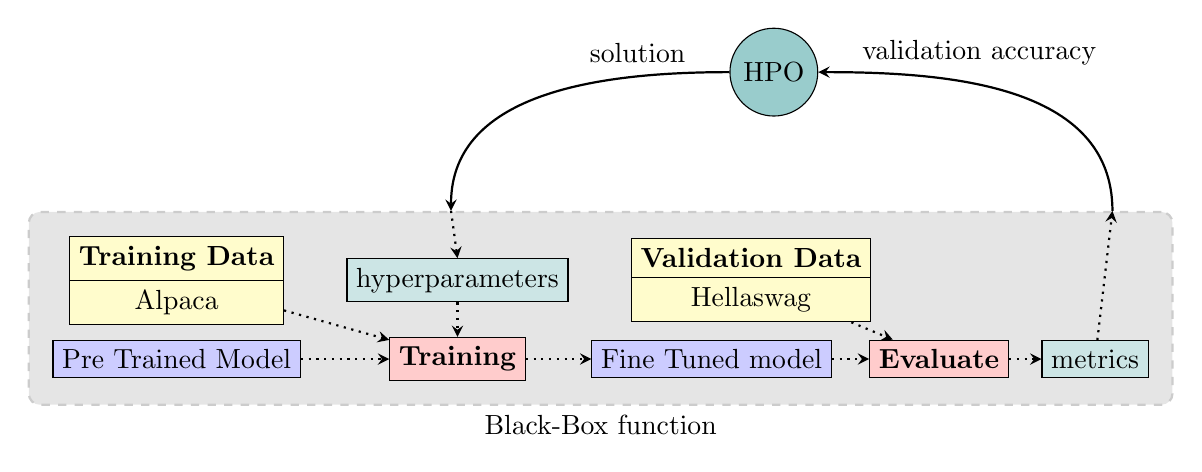
\begin{tikzpicture}
    \tikzstyle{data}=[rectangle split, rectangle split parts = 2,draw,text centered, fill=yellow!20]
    \tikzstyle{model} = [rectangle, draw, text centered, fill = blue!20]
    \tikzstyle{function} = [rectangle, draw, text centered, fill = red!20, font = \bfseries]
    \tikzstyle{metrics} = [rectangle, text centered, draw, fill=teal!20]
    
\tikzstyle{dot_arrow} = [thick,dotted,->,>=stealth]

\node (train_data) [data]
    {
        \textbf{Training Data}
        \nodepart{second} Alpaca};  

\node (PT_model)[model, below of = train_data]{Pre Trained Model };

\node (training) [function, right of = PT_model, anchor = west, xshift = 1.7cm]{Training};

\node (hp) [metrics, above of = training]{hyperparameters};

\node (FT_model) [model, right of = training, anchor = west, xshift = 0.7cm]{Fine Tuned model};

\node (val_data) [data, above of = FT_model, xshift = 0.5cm]
    {
        \textbf{Validation Data}
        \nodepart{second} Hellaswag}; 
        
\node (evaluate) [function, right of = FT_model, anchor = west, xshift = 1cm]{Evaluate};

\node (metrics) [metrics, right of = evaluate, anchor = west, xshift = 0.3cm]{metrics};


\begin{scope}[on background layer]
    \node(bbfunction)[draw, thick,fill=black!10,draw=black!20, dashed, rounded corners, fit=(train_data) (PT_model) (training) (FT_model)(val_data)(evaluate)(metrics), inner sep=0.3cm, label=below:{Black-Box function  }] {};
\end{scope}

\draw [dot_arrow] (train_data) -- (training);
\draw [dot_arrow] (PT_model) -- (training);
\draw [dot_arrow] (hp) -- (training);
\draw [dot_arrow] ([xshift = -1.9cm]bbfunction.north) -- (hp.north);
\draw [dot_arrow] (training) -- (FT_model);
\draw [dot_arrow] (val_data) -- (evaluate);
\draw [dot_arrow] (FT_model) -- (evaluate);
\draw [dot_arrow] (evaluate) -- (metrics);
\draw [dot_arrow] (metrics) -- ([xshift = 6.5cm]bbfunction.north);

\node (hpo) [circle, above of = bbfunction, yshift = 2cm,xshift=2.2cm, draw, fill = teal!40]{HPO};
\node [left of = hpo, yshift = 0.25cm, anchor = east]{solution};
\node [right of = hpo, yshift = 0.25cm,anchor = west]{validation accuracy};

%\draw [thick,->,>=stealth]    ([xshift = 6.25cm]bbfunction.north) to[out=90,in=-5] (hpo.east);
\draw [thick,<-,>=stealth]     (hpo.east)to[out=0,in=90] ([xshift = 6.5cm]bbfunction.north);
\draw [thick,->,>=stealth]     (hpo.west) to[out=180,in=90] ([xshift = -1.9cm]bbfunction.north);




\end{tikzpicture}
                }
                \caption{HPO workflow}
           \end{figure}  
           \end{column}
                
       \end{columns}

\end{frame}

%---------------------------------- Review Summary -------------------------------
\begin{frame}{Related Works}
    \begin{figure}
        \resizebox{0.9\textwidth}{!}{
            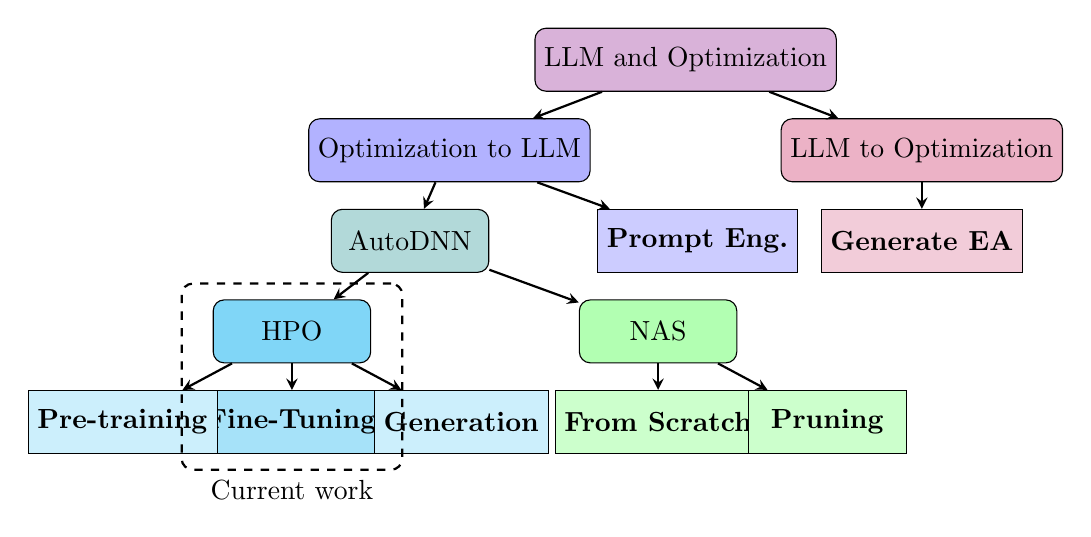
\begin{tikzpicture}[node distance = 1.15cm]

\tikzstyle{field} = [rectangle,rounded corners, minimum width=2cm, minimum height=0.8cm, text centered, draw=black]
\tikzstyle{art} = [minimum width=2cm, minimum height=0.8cm, text centered, draw=black, fill=blue!30]
\tikzstyle{arrow} = [thick, ->, >=stealth]


% base
\node (base)[field, fill = violet!30]{LLM and Optimization};

% lvl 1
\node (opt_llm)[field, below of = base, xshift = -3cm, fill = blue!30]{Optimization to LLM};

\node (llm_opt)[field, below of = base, xshift = 3cm, fill = purple!30]{LLM to Optimization};

% lvl 2
\node (autodnn)[field, below of = opt_llm, xshift = -0.5cm, fill=teal!30]{AutoDNN};
\node(prompt)[art,right of = autodnn, xshift = 2.5cm, fill = blue!20]{
    \textbf{Prompt Eng.}
};
\node (gen_ea)[art, below of = llm_opt, fill = purple!20]{
    \textbf{Generate EA}
};

% lvl 3
\node (hpo)[field, below of = autodnn, xshift = -1.5cm, fill = cyan!50]{HPO};
\node (nas)[field, right of = hpo, xshift = 3.5cm, fill = green!30]{NAS};

% lvl4 hpo

\node (hpo_ft)[art, below of = hpo, fill = cyan!35]{
    \textbf{Fine-Tuning}
};
\node (hpo_pt)[art, left of = hpo_ft, xshift = -1cm, fill = cyan!20]{
    \textbf{Pre-training}
};
\node (hpo_gen)[art, right of = hpo_ft,xshift = 1cm, fill = cyan!20]{
    \textbf{Generation}
};
% lvl4 nas
\node (nas_scratch)[art, below of = nas, fill = green!20]{
    \textbf{From Scratch}
};
\node (nas_pruning)[art, right of = nas_scratch,xshift = 1cm, fill = green!20]{
    \textbf{Pruning}
};

% arrows
\draw[arrow] (base) -- (opt_llm);
\draw[arrow] (base) -- (llm_opt);

\draw[arrow] (opt_llm) -- (autodnn);
\draw[arrow] (opt_llm) -- (prompt);
\draw[arrow] (llm_opt) -- (gen_ea);

\draw[arrow] (autodnn) -- (hpo);
\draw[arrow] (autodnn) -- (nas);

\draw[arrow] (hpo) -- (hpo_pt);
\draw[arrow] (hpo) -- (hpo_ft);
\draw[arrow] (hpo) -- (hpo_gen);

\draw[arrow] (nas) -- (nas_scratch);
\draw[arrow] (nas) -- (nas_pruning);

% fitting box
\node (current)[draw,thick, dashed, rounded corners, 
    fit = (hpo)(hpo_ft), inner sep = 0.2cm,
    label = below :{Current work}]{};

\end{tikzpicture}
        }
        \caption{Summary of links between LLM and Optimization}
    \end{figure}
    
    
\end{frame}
%%%%%%%%%%%%%%%%%%%%%%%%%%%%%%%%%%%%%%%%%%%%%%%%%%%%%%%

%%%%%%%%%%%%%%%%%%%%%%%%%%%%%%%%%%%%%%%%%%%%%%%%%%%%%%%
% \section{Review of Related Works}
% \frame{\sectionpage}
% \include{frames/review}
%%%%%%%%%%%%%%%%%%%%%%%%%%%%%%%%%%%%%%%%%%%%%%%%%%%%%%%

%%%%%%%%%%%%%%%%%%%%%%%%%%%%%%%%%%%%%%%%%%%%%%%%%%%%%%%
\section{Problem Definition}
\frame{\sectionpage}
%---------------------------------- Problem definition -------------------------------
\begin{frame}{Problem Definition}
   

    \begin{columns}
    
        \begin{column}[t]{0.45\textwidth}
            

            \begin{block}{Problem Formulation}
                The HPO problem can be defined as 
                \begin{equation}
                \eta^* \in \arg\min_{\eta \in \mathcal{H}} \mathcal{F}(\eta) 
                \end{equation}
            \end{block}

            This function can be characterized as an \large\textbf{expensive, mixed-variable, noisy, blackbox} function.
            \end{column}
        
        \begin{column}[t]{0.45\textwidth}
            \begin{block}{3 phases of an optimization problem}
                \begin{itemize}
                    \item \textbf{Search Space $\mathcal{H}$} : all variables and how to handle them
                    \item \textbf{Search Strategy $\arg\min$} : how to search for the minimum of the function
                    \item \textbf{Performance Evaluation Strategy $\mathcal{F}(.)$} : how to evaluate a given solution
                \end{itemize}
            \end{block}

        \end{column}
         
  \end{columns}
\end{frame}


%------------------------------------ Search Space ---------------------------
\begin{frame}{Search Space}


    \begin{block}{Hyperparameters}
    
        \begin{table}[h!]
            \centering
            \begin{tabular}{|c|c|c|c|c|}
                \hline
                \multirow{2}{*}{\textbf{ Hyperparameters }} & \multicolumn{2}{|c|}{\textbf{Optimization range}} &\multirow{2}{*}{\textbf{ Type }}& \multirow{2}{*}{\textbf{ Conversion }} \\
                \cline{2-3}
                 & \textbf{ Lower Bound } & \textbf{ Upper Bound } & & \\
                \hline
                \textbf{Learning Rate} & $-10$ & $-1$ & log. & $f(x) = 10^{x}$ \\
                \hline
                \textbf{LoRA Rank} & 1 & 64 &int. &$f(x) = \text{round}(x)$ \\
                \hline
                \textbf{LoRA scale ($\alpha$)} &1 & 64 & int. &$f(x) = \text{round}(x)$ \\
                \hline
                \textbf{LoRA Dropout} & 0 & 0.5 & cont.& $f(x) = x$ \\
                \hline
                \textbf{Weight Decay} & $-3$ & $-1$ &log.& $f(x) = 10^{x}$  \\
                \hline
            \end{tabular}
            \caption{Summary of Hyperparameter Search Space}
            \label{tab:hyperparam_table}
        \end{table}
        
    \end{block}
    
    
    \begin{itemize}
        \item Conversion and naming convention is taken from LitGPT framework.
        \item Variable conversion for handling mixed-variables with continuous algorithms
        \item No \textit{A-priori} knowledge on hyperparameters importance
    \end{itemize}
\end{frame}


%---------------------------------- Search Strategy  -------------------------------
\begin{frame}{Search Strategy}
    Algorithms for LLM HPO are \textit{Global Optimization} algorithms. Can be classified as : 

    \begin{itemize}
        \item \textbf{Exploratory}(GS, Random Search, LHS) : sample the search space\\ \quad no exploitation, give a lower bound
        \item \textbf{Metaheuristics} (Genetic Algorithm, ILS, PSO) : bio-inspired heuristics \\ \quad evaluation greedy, cannot be used for expensive function
        \item \textbf{Surrogate-Model based Optimization} (Bayesian Optimization with Gaussian Process, TS) : \\ \quad Use a surrogate to enhance exploitation - innate sequential nature, strong exploitation
        \item \textbf{Partition-Based Optimization}(FDA, SOO, DiRect) : partition the search space \\ \quad massively parallel, slow convergence
    \end{itemize}


\end{frame}

%---------------------------------- Performance Evaluation Strategy -------------------------------

\begin{frame}{Performance Evaluation Strategy}
    \begin{block}{Evaluation context}
    In this part, there are many options, like the number of epochs (if not an hyperparameters), the precision of the model, the datasets of training or evaluation. 
        
    \end{block}
    \begin{block}{Objective function}
        2 ways to evaluate LLM Fine-Tuning : 
        \begin{itemize}
            \item \textbf{Loss (validation/test)} : dataset and model dependant, difficult to compare to other models.
            \item \textbf{Accuracy on Benchmark dataset (GLUE, MMLU)} : can be used to compare to other models throughout the training. 
        \end{itemize}
    \end{block}

    \begin{block}{Complementary approaches}
        \begin{itemize}
            \item Multi-fidelity : reduce the cost and the reliability of early evaluations. (ex : BOHB algorithm)
        \end{itemize}
        
    \end{block}
    
\end{frame}
%%%%%%%%%%%%%%%%%%%%%%%%%%%%%%%%%%%%%%%%%%%%%%%%%%%%%%%

%%%%%%%%%%%%%%%%%%%%%%%%%%%%%%%%%%%%%%%%%%%%%%%%%%%%%%%
\section{Design and Implementation}
\frame{\sectionpage}


%---------------------------------- BO-GP -------------------------------
\begin{frame}{SMBO : Bayesian-Optimization based on Gaussian-Process (BO-GP)}
    \begin{columns}
        \begin{column}{0.4\textwidth}

            \begin{block}{Principle :}
                Iterate these two steps over budget : 
                \begin{enumerate}
                    \item Build a surrogate of the objective function
                    \item Optimize the surrogate to find the most promising point to evaluate
                \end{enumerate}
                
                
            \end{block}
            
        \end{column}        
        \begin{column}{0.5\textwidth}
            \begin{figure}
                \centering
                \usepgfplotslibrary[fillbetween]
\begin{tikzpicture}[domain = 0:5,scale = 0.7]

    \begin{axis}[
        legend pos=outer north east,
        ymin = 2.5,ymax=5, 
        xmin = 0, xmax = 5,
        x=40,
        y =55
    ]
    % plot function
    \addplot [no markers, blue, dashdotted, thick,visible on =<-3>] {sin(\x r)^2+sqrt(\x+8)};
    \addlegendentry[visible on =<-3>]{$f(x)$}

    % Add sampling
    % LHS
    \addplot [blue, only marks, mark = *,visible on =<2-3>] table {assets/tikz_picture/gaussian_process/lhs.dat};
    \addlegendentry[visible on =<2-3>]{$LHS(\Omega)$}

    
    \draw[color=teal!50, dashed,visible on =<2>](axis cs:1.25, -5) -- (axis cs:1.25, 27);
    \draw[color=teal!50, dashed,visible on =<2>](axis cs:2.5, -5) -- (axis cs:2.5, 27);
    \draw[color=teal!50, dashed,visible on =<2>](axis cs:3.75, -5) -- (axis cs:3.75, 27);

    % Surrogate
    \addplot [red,visible on =<3-3>] table {assets/tikz_picture/gaussian_process/mean.dat};
    \addlegendentry[visible on =<3-3>]{$\hat{f}(x)$}
    % UCB
    \addplot [violet,dashed,visible on =<3>] table {assets/tikz_picture/gaussian_process/ucb.dat};
    \addlegendentry[visible on =<3>]{$UCB$ }
    % LCB
    \addplot [violet,dashed,visible on =<3>] table {assets/tikz_picture/gaussian_process/lcb.dat};
    \addlegendentry[visible on = <3>]{$LCB$}

    % Optimize UCB
    \addplot [violet,visible on =<4>] table {assets/tikz_picture/gaussian_process/ucb.dat};
    \addlegendentry[visible on =<4>]{$UCB$ }

    % Local Search 1 : 
        \addplot [violet,visible on =<4>, mark = triangle*,mark size = 3, mark indices = {16,20,25},only marks, mark options = {rotate = 90, color = blue!50}] table {assets/tikz_picture/gaussian_process/ucb.dat}; 
        \addplot [violet,visible on =<4>, mark = triangle*,mark size = 4, mark indices = {27},only marks, mark options = { color = blue}] table {assets/tikz_picture/gaussian_process/ucb.dat};
    % Local Search 2
        \addplot [violet,visible on =<4>, mark = triangle*,mark size = 3, mark indices = {40,35,45},only marks, mark options  = {rotate = 180, color = teal!50}] table {assets/tikz_picture/gaussian_process/ucb.dat};
        \addplot [violet,visible on =<4>, mark = triangle*,mark size = 4, mark indices = {33},only marks, mark options = {color = teal}] table {assets/tikz_picture/gaussian_process/ucb.dat};
    % Local Search 3
        \addplot [violet,visible on =<4>, mark = triangle*,mark size = 3, mark indices = {60,65,70,75},only marks, mark options = {rotate = 90, color = red!50}] table {assets/tikz_picture/gaussian_process/ucb.dat}; 
        \addplot [violet,visible on =<4>, mark = triangle*,mark size = 4, mark indices = {79},only marks, mark options  = {color = red}] table {assets/tikz_picture/gaussian_process/ucb.dat};
    % Best final
    \draw[color=red!50, dashed,visible on =<4>](axis cs:0.79*5, -5) -- (axis cs:0.79*5, 27);



    \end{axis} 

    %\onslide<2->\node[font = \small] at (9,2){Etape :};

    %\onslide<2>{\node[anchor = west,font = \small] at (9.6,2){Echantillonage};}
    %\onslide<3>{\node[anchor = west,font = \small] at (9.6,2){Fit GP};}
    %\onslide<4>{\node[anchor = west,font = \small] at (9.6,2){Opt. UCB};}

\end{tikzpicture}
                \caption{Illustration of BO-GP Algorithm}
            \end{figure}
        \end{column}
    \end{columns}
    
\end{frame}

%---------------------------------- SOO -------------------------------
\begin{frame}{PBO : Simultaneous Optimistic Optimization(SOO)}
    \begin{columns}[b]
        \begin{column}{0.4\textwidth}
            \begin{block}{Principle\footnote[6]{Munos, Rémi. « Optimistic Optimization of a Deterministic Function without the Knowledge of its Smoothness ». 2011} : }
                \begin{itemize}
                    \item K-inary partition of the space
                    \item Evaluate the center of each partition
                    \item Expand a maximum of one node by iteration / by depth
                \end{itemize}
            \end{block}
            
        % \vspace*{35pt}
        \end{column}    

        \begin{column}[b]{0.27\textwidth}
            \begin{figure}[h]
                \centering
                \resizebox{\textwidth}{!}{
                    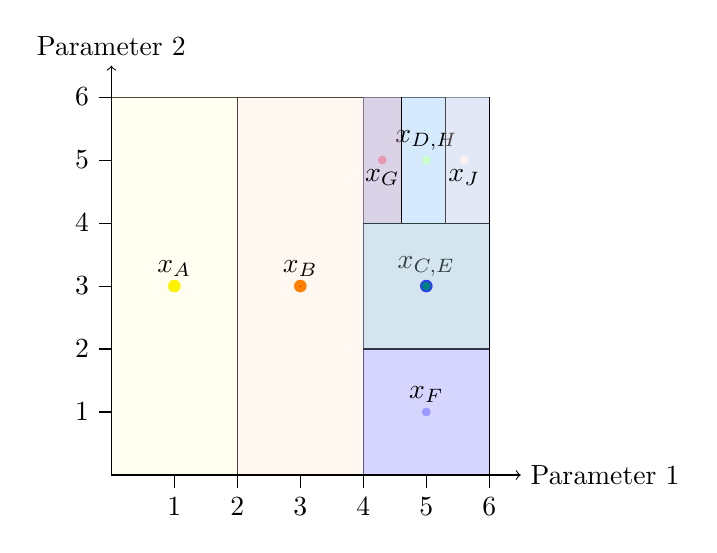
\begin{tikzpicture}[scale=0.8]

    % Define the grid
    \draw[step=6,black,very thin] (0,0) grid (6,6);

    
    % first decomposition
    \draw (2,0) -- (2,6) ;
    \draw (4,0) -- (4,6);
        % point A
        \fill[yellow!20, opacity = 0.3] (0.0,0) rectangle (2,6);
        \fill[fill = yellow] (1,3) circle (0.1) node[above]{$x_A$};  % Point in the first square
        
        % point B
        \fill[orange!20, opacity = 0.3] (2,0) rectangle (4,6);
        \fill[fill = orange] (3,3) circle (0.1) node[above]{$x_B$};  % Point in the first square
        % point C
        \fill[blue!20, opacity = 0.3] (4,0) rectangle (6,6);
        \fill[fill = blue] (5,3) circle (0.1) node[above]{$x_{C,E}$};  % Point in the first square

    % second decomposition
    \draw (4,2) -- (6,2);
    \draw (4,4) -- (6,4);
      % point D
      \fill[cyan!40, opacity = 0.3] (4,4) rectangle (6,6);
      \fill[fill = cyan!40] (5,5) circle (0.07) node[above]{$x_{D,H}$} ;  % Point in the first square
      %point E
      \fill[teal!40, opacity = 0.3] (4,2) rectangle (6,4);
      \fill[fill = teal] (5,3) circle (0.07) ;  % Point in the first square
      %point F
      \fill[blue!40, opacity = 0.3] (4,0) rectangle (6,2);
      \fill[fill = blue!40] (5,1) circle (0.07) node[above]{$x_F$} ;  % Point in the first square

    % second decomposition
    \draw (4.6,4) -- (4.6,6);
    \draw (5.3,4) -- (5.3,6);
      %point G
      \fill[purple!40, opacity = 0.3] (4,4) rectangle (4.6,6);
      \fill[fill = purple!40] (4.3,5) circle (0.07) node[below]{$x_G$} ;  % Point in the first square
      %point H
      %\fill[green!40, opacity = 0.3] (4.6,4) rectangle (5.3,6);
      \fill[fill = green!20] (5,5) circle (0.07);  % Point in the first square
      %point J
      \fill[pink!40, opacity = 0.3] (5.3,4) rectangle (6,6);
      \fill[fill = pink!20] (5.6,5) circle (0.07) node[below]{$x_J$} ;  % Point in the first square
    

    % Draw red points
    \fill[red] (3,3) circle (0.01);  % Point in the first square

    
    % Draw the axes
    \draw[->] (0,0) -- (6.5,0) node[right] {Parameter 1};
    \draw[->] (0,0) -- (0,6.5) node[above] {Parameter 2};
    
    % Add ticks and labels
    \foreach \x in {1,2,3,4,5,6} {
      \draw (\x,0) -- (\x,-0.2) node[below] {\x};
      \draw (0,\x) -- (-0.2,\x) node[left] {\x};
    }
    
\end{tikzpicture}
                }
                \caption{SOO Partition}
            \end{figure}
        \end{column}

        \begin{column}[b]{0.33\textwidth}
            \begin{figure}[h]
                \centering
                \resizebox{\textwidth}{!}{
                    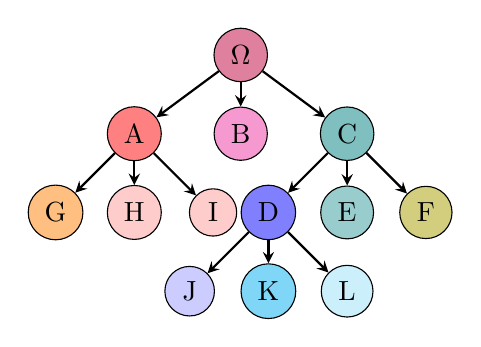
\begin{tikzpicture}[]
    \tikzstyle{space} = [circle, minimum width=0.6cm,text centered, draw=black]
    \tikzstyle{arrow} = [thick,->,>=stealth]

      \node(space)[space, fill = purple!50]{$\Omega$};


 
        %depth 1
        \node(B)[space, fill = magenta!40, below of = space, yshift = -0cm]{B};
        \node(A)[space, fill = red!50, left of = B, xshift = -10pt]{A};
        \node(C)[space, fill = teal!50,  right of = B, xshift = 10pt]{C};
        \draw[arrow] (space) -- (A);
        \draw[arrow] (space) -- (B);
        \draw[arrow] (space) -- (C);
    
    \onslide<2->{ % First loop
    %depth 1
    \node(E)[space, fill = teal!40, below of = C, yshift = -0cm]{E};
    \node(D)[space, fill = blue!50, left of = E]{D};
    \node(F)[space, fill = olive!40,  right of = E]{F};
    \draw[arrow] (C) -- (E);
    \draw[arrow] (C) -- (D);
    \draw[arrow] (C) -- (F);
    }

    \onslide<3->{
    %depth 2
    \node(H)[space, fill = red!20, below of = A]{H};
    \node(G)[space, fill = orange!50, left of = H]{G};
    \node(I)[space, fill = pink!80,  right of = H]{I};
    \draw[arrow] (A) -- (G);
    \draw[arrow] (A) -- (H);
    \draw[arrow] (A) -- (I);

    \node(K)[space, fill = cyan!50, below of = D]{K};
    \node(J)[space, fill = blue!20, left of = K]{J};
    \node(L)[space, fill = cyan!20,  right of = K]{L};
    \draw[arrow] (D) -- (J);
    \draw[arrow] (D) -- (K);
    \draw[arrow] (D) -- (L);
    }
    
    

\end{tikzpicture}
                }
                \caption{SOO Tree}
            \end{figure}
        \end{column}
    \end{columns}
\end{frame}

%---------------------------------- BaMSOO -------------------------------
\begin{frame}{Hybridization : Bayesian Multi-Scale Optimistic Optimization (BaMSOO)}
    \begin{columns}
        \begin{column}{0.55\textwidth}
            \begin{block}{Principle\footnote[7]{Wang et al. « Bayesian Multi-Scale Optimistic Optimization ». 2014} : }
                \begin{itemize}
                    \item SOO partitionning
                    \item Use a Gaussian process to enhance the scoring
                \end{itemize}
                Objective : prevent unpromising evaluations
                
            \end{block}
            
            \begin{block}{BaMSOO Scoring $g(x)$ :}
                \begin{itemize}
                    \item \textbf{If} $UCB(x) > f^+$ : {\color{gray} // \small x has potential to beat $f^+$}
                        \begin{itemize}
                            \item $g(x) = f(x)$ {\color{gray} // \small score $x$ using $f(x)$}
                        \end{itemize}
                    \item \textbf{Else } :
                        \begin{itemize}
                            \item $g(x) = LCB(x)$ {\color{gray} // \small score $x$ using $LCB(x)$}
                        \end{itemize}


                \end{itemize}
                
            \end{block}
            
        \end{column}        
        \begin{column}{0.45\textwidth}
            \begin{figure}[h]
                \centering
                \begin{algorithm}
\caption{BamSOO}
\label{algo:bamsoo}
\begin{algorithmic}[1]
\Require\\
$\Omega$: Continuous search space \\
$f$: Objective function  \Comment{train and validate the model}\\
$K$ : number of section of the space\\
$n_{max}$ : budget of evaluation \\
$K_D$ : Kernel function\\

\State $x_{0,0} \gets center(\Omega)$ 
\State  $g_{0,0} \gets    f(x_{0,0})$
\State $\mathcal T_1 = \{x_{0,0},g_{0,0},\Omega\}$\Comment{Initiate the tree}
\State  $f^+ \gets g_{0,0}$
\State $n \gets 1$ \Comment{nodes index}
\State $t \gets 1$ \Comment{evaluation index}
\State $\mathcal D_1 = \{x_{0,0},g_{0,0}\}$ \Comment{list of evaluated points}
\\

\While{$t < n_{max}$}
    \State $\nu_{max} \gets - \infty$
    \For{$h=0 \textbf{ to } depth(\mathcal T_n)$}
        \State $j \gets \arg \max_{j \in \{j | (h,j) \in L_n\}} g_{h,j}$
        \If{$g_{h,j} > \nu_{max}$}
            \State $\Omega_{h+1,j+1},\dots,\Omega_{h+1,j+K} \gets section(\Omega_{h,j},K)$
            \For{$i=1$ \textbf{to }$K$}
                \State $\mu,\sigma \gets GP(\mathcal D_t,K_D)$
                \State $N \gets N+1$
                \State $x_{h+1,j+i} \gets center(\Omega_{n})$

                \If{$\mathcal{UCB}(x_{h+1,j+i},\mu,\sigma) \geq f^+$}
                    \State $g_{h+1,j+i} \gets f(x_{h+1,j+i}) $
                    \State $t \gets t+1$
                \Else
                    \State $g_{h+1,j+i} \gets \mathcal{LCB}(x_{h+1,j+i},\mu,\sigma) $
                \EndIf

                \If{$g_{h+1,j+i} > f^+$}
                    \State $f^+ \gets g_{h+1,j+i} $
                \EndIf         
                \State $n \gets n+1$               
                \State $\mathcal T_n \gets \{(x_{h+1,j+i},f_{h+1,j+i},\Omega_{h+1,j+i})\}$  
            \EndFor  
            \State $\nu_{max} \gets g_{h,j}$
        \EndIf
    \EndFor
\EndWhile\\
\Return best of $x_{h,j},g(x_{h,j})$
\end{algorithmic}
\end{algorithm}
                \caption{Illustration of BaMSOO Algorithm}
            \end{figure}
        \end{column}
    \end{columns}
\end{frame}

%---------------------------------- Evaluation Function -------------------------------
\begin{frame}{Evaluate the solution}
    Use LitGPT framework with it's CLI to perform an evaluation of a solution. All models and datasets are taken from HuggingFace Hub.


    \begin{columns}
        \begin{column}[t]{0.45\textwidth}
            \begin{block}{Training}
                \begin{itemize}
                    \item Model : Llama-3.2-1B\footnote[2]{Touvron et al. « LLaMA: Open and Efficient Foundation Language Models »,2023}
                    \item dataset : Alpaca\footnote[3]{Hashimoto et al. « Stanford Alpaca: An Instruction-following LLaMA model ». 2024}
                    \item 1 epochs of training
                    \item Fully Sharded Data Parallelism (FSDP) as distributed strategy
                \end{itemize}
            \end{block}
        \end{column}
        \begin{column}[t]{0.45\textwidth}
            \begin{block}{Evaluating}
                Based on lm\_eval library
                \begin{itemize}
                    \item validation dataset : Hellaswag\footnote[4]{Zellers et al. « HellaSwag: Can a Machine Really Finish Your Sentence? » 2019.
                    }
                    \item testing dataset : MMLU\footnote[5]{Hendrycks et al. « Measuring Massive Multitask Language Understanding ». 2021
                    }
                \end{itemize}
            \end{block}
        \end{column}
    \end{columns}

    
\end{frame}
%%%%%%%%%%%%%%%%%%%%%%%%%%%%%%%%%%%%%%%%%%%%%%%%%%%%%%%

%%%%%%%%%%%%%%%%%%%%%%%%%%%%%%%%%%%%%%%%%%%%%%%%%%%%%%%
\section{Computation Experiments}
\frame{\sectionpage}
\begin{frame}{Experimental Setup}

    \begin{block}{Experimental testbed}
        Experiments presented in this paper were carried out using the Grid'5000 testbed, supported by a scientific interest group hosted by Inria and including CNRS, RENATER and several Universities as well as other organizations (see https://www.grid5000.fr).
    \end{block}
    
    \begin{block}{Hardware and budget allocated}
        One evaluation on chuc cluster, using 4*A100 40G of VRAM GPU, is taking around 40 minutes. Each algorithms have a budget of 50 evaluations, including the 10 sampling evaluation of BO. 
    \end{block}


    
    
\end{frame}
%---------------------------------- Sampling experiment -------------------------------
\begin{frame}{Sampling experiment : Latin Hypercube Sampling}
    
    \begin{columns}
        \begin{column}{0.4\textwidth}
            
            Objective : Explore the space and define a lower bound for next experiments

            \begin{figure}
                \centering

                \input{imgs/experiments/lhs/lhs.tex}
                \caption{LHS illustration with $g=5$ samples}
            \end{figure}
            
        \end{column}

        \begin{column}{0.6\textwidth}
            \begin{figure}
                \centering
                \includegraphics[width = \textwidth]{imgs/experiments/lhs/lhs.png}     
                \caption{Results of LHS Experiment\footnote[5]{ \textit At left : correlation between metrics and hyperparameters // At right : metrics distribution}}         
            \end{figure}
            
        \end{column}
\end{columns}  

\end{frame}



%---------------------------------- Bayesian Optimization -------------------------------
\begin{frame}{Results : Bayesian Optimization} 
    
    \begin{columns}
    
        \begin{column}{0.6\textwidth}
            \begin{block}{Score over time}
                \begin{figure}
                    \centering
                    \begin{tikzpicture}[domain = 0:50,scale = 0.7]
    \tikzstyle{point} = [only marks, mark = triangle*, mark size = 3, opacity = 0.5]
    \begin{axis}[
        legend pos=south east,
        ymin = 0.2,
        x=3.2,
        y =450
    ]
    \addplot [blue,point] table {imgs/experiments/bo/bo_hs.dat};
    \addlegendentry{$f(x)$}

    \draw[color=red, dashed](axis cs:10,0) -- (axis cs:10,0.5);




    \end{axis}
\end{tikzpicture}
                    \caption{Results on validation dataset for BO-GP Algorithm}
                \end{figure}
            
            \end{block}   
        \end{column}

        \begin{column}{0.4\textwidth}
            \begin{block}{Results}
                Hellaswag($D_{val}$) Best score : 47,91\%        
            \end{block}

            \begin{block}{Behavior}

                \begin{itemize}
                    \item Fast convergence after sampling phase
                    \item Few shots emphasizing exploration with lower score
                \end{itemize}
                
                
            \end{block}
             
        \end{column}
    \end{columns}    
\end{frame}

%---------------------------------- SOO -------------------------------
\begin{frame}{Results : SOO} 
    
    \begin{columns}
    
        \begin{column}{0.6\textwidth}
            \begin{block}{Score over time}
                \begin{figure}
                    \centering
                    \begin{tikzpicture}[domain = 0:50,scale = 0.7]
    \tikzstyle{point} = [only marks, mark = triangle*, mark size = 3, opacity = 0.5]
    \begin{axis}[
        legend pos=south east,
        ymin = 0.2,
        x=3.2,
        y =450
    ]
    \addplot [red,point] table {imgs/experiments/soo/soo_hs.dat};
    \addlegendentry{$f(x)$}




    \end{axis}
\end{tikzpicture}
                    \caption{Results on validation dataset for SOO Algorithm}
                \end{figure}
            
            \end{block}   
        \end{column}

        \begin{column}{0.4\textwidth}
            \begin{block}{Results}
                Hellaswag($D_{val}$) Best score : 47.84\%        
            \end{block}

            \begin{block}{Behavior}

                \begin{itemize}
                    \item A lot of low score evaluation, due to one hyperparameter
                    \item maximum depth of 8 (only 2 points with depth = 8)
                \end{itemize}

            \end{block}
             
        \end{column}
    \end{columns}    
\end{frame}


%---------------------------------- BaMSOO -------------------------------
\begin{frame}{Results : BaMSOO} 
    
    \begin{columns}
    
        \begin{column}{0.6\textwidth}
            \begin{block}{Score over time}
                \begin{figure}
                    \centering
                    \input{imgs/experiments/bamsoo/bamsoo_res.tex}
                    \caption{Results on validation dataset for BaMSOO Algorithm}
                \end{figure}
            
            \end{block}   
        \end{column}

        \begin{column}{0.4\textwidth}
            \begin{block}{Results}
                Hellaswag($D_{val}$) Best score : 47.84\% \\
                Do not achieve to overperform SOO best score   
            \end{block}

            \begin{block}{Behavior}

                \begin{itemize}
                    \item Prevent SOO unpromising evaluation (16 approximated evaluations)
                    \item maximum depth of 8 (8 points with depth = 8)
                \end{itemize}

            \end{block}
             
        \end{column}
    \end{columns}    
\end{frame}



%%%%%%%%%%%%%%% COMPARISON %%%%%%%%%%%%%%
\begin{frame}{Comparison and analysis}

    \begin{columns}
    
        \begin{column}{0.45\textwidth}

            \begin{block}{Analysis}
                \begin{itemize}
                    \item Upper Bound on Hellaswag is irrelevant
                    \item Only BO-GP beat LHS 
                    \item with more high-performing solution, BaMSOO overperform SOO on MMLU
                \end{itemize}
                
            \end{block}\vspace*{-10pt}
            
            \begin{block}{Results}
                \begin{table}[h!]
    \centering
    \begin{tabular}{|c||c|c|}
    \hline
       & Hellaswag & MMLU\\
    \hline\hline
       Lower Bnd$^1$  & 47.90 & 37.61 \\
       Upper Bnd$^2$  & \textit{41.5} & 49.3 \\
    \hline
       BO-GP  & \textbf{47.91} & \textbf{38.11} \\
       SOO  & 47.84 & 37.42 \\
       BaMSOO  & 47.84 & 37.50 \\
    \hline
    \end{tabular}
    \caption{Bound and best score for datasets (val and test)}
\end{table} 
\vspace*{-15pt}{\footnotesize 1 : LHS results; 2 : Meta Fine tuning }
            \end{block}
            
            
            
        \end{column}

        \begin{column}{0.45\textwidth}
            \begin{block}{Score over time on testing dataset}
                \begin{figure}
                    \centering
                    \begin{tikzpicture}[domain = 0:50,scale = 0.7]
    \tikzstyle{point} = [only marks, mark = triangle*, mark size = 3, opacity = 0.5]
    \begin{axis}[
        legend pos=south east,
        ymin = 0.2,
        x=3.2,
        y =700
    ]
    \addplot [blue,point, visible on = <1> ] table {assets/tikz_picture/global_results/bo_mmlu.dat};
    \addlegendentry{BO}

    \addplot [red, point, visible on = <2>] table {assets/tikz_picture/global_results/soo_mmlu.dat};
    \addlegendentry{SOO}

    \addplot [violet, point, visible on = <3>] table {assets/tikz_picture/global_results/bamsoo_mmlu.dat};
    \addlegendentry{BaMSOO}



    \addplot [blue,point, visible on = <4>] table {assets/tikz_picture/global_results/bo_mmlu.dat};
    \addplot [red, point, visible on = <4>] table {assets/tikz_picture/global_results/soo_mmlu.dat};
    \addplot [violet, point, visible on = <4>] table {assets/tikz_picture/global_results/bamsoo_mmlu.dat};




    \end{axis}
\end{tikzpicture}
                    \caption{Results on testing dataset for the three algorithms}
                \end{figure}
            
            \end{block}  
             
        \end{column}
    \end{columns}    

\end{frame}
%%%%%%%%%%%%%%%%%%%%%%%%%%%%%%%%%%%%%%%%%%%%%%%%%%%%%%%


\section{Conclusions and Perspectives}
\frame{\sectionpage}
\begin{frame}{Conclusions}

\begin{itemize}
    \item With limited budget, BO-GP demonstrated exceptional efficiency, quickly converging to high-performing solutions. 
    \item BaMSOO succed to fasten SOO convergence by preventing unpromising evaluations.
    \item Lay groundwork for using PBO algorithms, enhance with BO-GP to deal with LLM Fine-Tuning
\end{itemize}


\end{frame}

\begin{frame}{Perspectives}

    \begin{columns}
        \begin{column}{0.45\textwidth}

            \begin{block}{Extend experiments on the application}
                \begin{itemize}
                    \item Extend search space (add hyperparameters, bigger range...)
                    \item Use more models/datasets
                    \item Make a distributed implementation
                \end{itemize}
            \end{block}
        \end{column}

        \begin{column}{0.45\textwidth}
            \begin{block}{Generalization of BaMSOO Hybridization}

                \begin{itemize}
                    \item explore parallelism of BO-GP based algorithms
                    \item Global Framework of \textit{Parallel Bayesian-enhanced Fractals Optimization} 
                \end{itemize}
            \end{block}
        \end{column}

    \end{columns}
    
\end{frame}


\begin{frame}[allowframebreaks]{Bibliography}
\printbibliography[]
\nocite{*}
\end{frame}






%%%%%%%%%%%%%%%%%%%%%%%%%%%%%%%%%%%%%%%%%%%%%%%%%%%%%%%

%% Le texte est modifiable en changeant \thankyou
\renewcommand{\thankyou}{Thank You.}
\frame{\merci}

%%%%%%%%%%%%%%%%%%%%%%%%%%%%%%%%%%%%%%%%%%%%%%%%%%%%%%% 

\end{document}

%%%%%%%%%%%%%%%%%%%%%%%%%%%%%%%%%%%%%%%%%%%%%%%%%%%%%%%
%%
%%%%%%%%%%%%%%%%%%%%%%%%%%%%%%%%%%%%%%%%%%%%%%%%%%%%%%%

